\documentclass[12pt,fleqn]{article}\usepackage{../../common}
\begin{document}
Oyun Teorisi ile Grup Kararları Tahmini

Bruce de Mesquita mutabakata / anlaşmaya varma / savaş konularında tahminler
yapabilen bir araştırmacı. Girdi olarak alttaki gibi bir veriyi alıp,

\begin{minted}[fontsize=\footnotesize]{python}
import pandas as pd
dfemis = pd.read_csv('emission.csv'); print dfemis
\end{minted}

\begin{verbatim}
         Actor  Capability  Position  Salience
0  Netherlands        0.08         4        80
1      Belgium        0.08         7        40
2   Luxembourg        0.03         4        20
3      Germany        0.16         4        80
4       France        0.16        10        60
5        Italy        0.16        10        60
6           UK        0.16        10        90
7      Ireland        0.05         7        10
8      Denmark        0.05         4       100
9       Greece        0.08         7        70
\end{verbatim}

onu hangi mutabakatın olacağı tahmini için kullanabiliyor. Üstteki veri bazı
ülkeler arasında orta boy arabalarda emisyon kontrolünü kaç sene sonra devreye
sokulacağı hakkında bir grup kararı. BDM'nin bu hesabı yapmak için iki yöntemi
var, birincisi yarı-Oyun Teorisel (quasi Game Theoretic), ikincisi tam Oyun
Teorik (ve daha kuvvetli bazı özellikleri var). Birinci model hakkında daha çok
dokümantasyon var, bu model ile BDM pek çok başarılı tahmine de imza attı bu
arada. Bu yazıda paylaşacağımız birinci model ve onun kodlaması.

Veride güç / beceri (capability), ve ilgi (salience) parametreleri var. Bunların
ne olduğu belli. Pozisyon üzerinde anlaşmazlık olan şeydir, her türlü karar
ilginç bir şekilde tek boyutlu bir skala üzerinden temsil edilebiliyor, yani bir
şey hiç istememek 0, çok istemek 100, ve arada tüm seçimler aradaki değerler
olabilir. Çok / az istemek arasındaki her nokta belli seçenek kombinasyonlarını
bile barındırıyor olabilir.

Oyunun sonucu ``evreler'' üzerinden işlenir. Her evrede aktörler güçleri
oranında diğer aktörleri kendi pozisyonlarına davet ediyorlar, ya da
etmiyorlar. Bir evrede her aktör pek çok diğer aktörden ``benim yanıma gel''
isteği almış olabilir, evre sonunda aktör bu tekliflerden (offer) kendisi için
en az değişim gerektirecek seçeneğe gidiyor (ilk başlangıç noktasına göre, bir
öncekine göre değil). Hoca bunu bu şekilde seçmiş ve iyi bir seçim bizce çünkü
doğa enerji israfını sevmez. İnsanlar da öyle!

Ortalamalar

Bir oyunun, herhangi bir evresi için, ağırlıklı ortalama ve ağırlıklı doruğu
(mode) hesaplanabilir. Ağırlıklı çünkü herkesin pozisyonunun basit ortalaması
değil, kişilerin ilgi ve gücü ile orantılı bir ortalama. Ağırlıklı ortalama için
formül

$$ \frac{\sum_{i=1}^{n} c_i s_i x_i}{\sum_{i=1}^{n} c_i s_i} $$

Ağırlıklı doruk için biraz takla lazım, önce tüm veriyi pozisyonlara göre
sıralarız, herkesin $c_is_i$ çarpımını hesaplayıp normalize ederiz, ve kümülatif
olarak bu rakamları toplarız. Hangi noktada 0.5'e erişilmiş ise o nokta
``ağırlıklı orta'' oluyor, ve o noktanın pozisyonu doruk olarak kabul
ediliyor. Hatırlanabileceği üzere basit doruk hesabı için, yani düz bir liste
sayı için, o sayılar sıralanıyordu, ve ortadaki sayı mode olarak
seçiliyordu. Burada aynı kavram sadece $c_i,s_i$ işin içinde.

\begin{minted}[fontsize=\footnotesize]{python}
import scholz
dfiran.Salience = dfiran.Salience/100.
game = scholz.Game(dfiran)
print 'ortalama', game.mean()
print 'mode', game.weighted_median()
\end{minted}

\begin{verbatim}
ortalama 54.3833734112
mode 50.0
\end{verbatim}

Her evrede hesaplanan ana formüller şunlar,

$$ E(U_{ij}|\textrm{teklif et}) = (1-s_j)U_{si} + s_jP_i^i U_{si} + s_j(1-P_i^i)U_{fi} $$

$$ E(U_{ij}|\textrm{teklif etme}) = QU_{sq} + (1-Q) \big( T U_{bi}) + (1-T)U_{wi} \big)$$

$$ E(U_{ij}) = E(U_{ij}|\textrm{teklif et}) - E(U_{ij}|\textrm{teklif etme}) $$

Teklif etmek bir diğer oyuncuyu pozisyonunu değiştirmesi için iknaya uğraşmak /
ona ``sormak'' (challange).  Formülerin bileşenlerini altta açacağız. Önce genel
faydadan başlayalım. Fayda (utility) $U_{ij}^i$ aktör $i$'nin kendi pozisyonuna
benzerliğe verdiği değerdir, diğer aktör $j$ uzaksa buna atanan fayda az,
yakınsa çoktur.

$$ U_{ij}^i = 1-2 \bigg| \frac{x_i - x_j}{x_{max}-x_{min}}\bigg|   $$

$U_{ii}^i$ doğal olarak 1 değerinde, aktör kendi pozisyonunda en çok
faydayı görüyor. 

Bir aktör bir diğer aktörü iknaya uğraşabilir. Bu durumda elde edeceği
fayda -başarılı olursa- aktörün kendi pozisyon faydası ve diğerinin
arasındaki uzaklığa oranlı görülebilir. Yani bana en uzak pozisiyondaki
birini ikna etmek bana en çok fayda getirir, daha yakın, daha az. Her
aktörün içinde olduğu risk $ 0 \le r_i \le 1$ olacak şekilde (ki risk ile
ne denmek istediğini ileride anlatacağız),

$$ U_{si}^i = 2 - 4 \bigg[ \frac{2-(U_{ii}^i - U_{ij}^i)}{4}  \bigg]^{r_i}$$

Kaybetme durumunda kaybedilen fayda $U_{fi}^i$ ise üstteki faydalar
çıkartmalarının ters çevirilmiş hali olarak düşünebilirim, bir anlamda ikna
edilmiş olma durumu olabilir bu, ikna ettiğimde kazandığıma göre
edildiğimde kaybederim, ve bu çıkarma işleminin ters çevirilmiş hali gibi
görülebilir, yani $ U_{ij}^i - U_{ii}^i$, o zaman

$$ U_{fi}^i = 2 - 4 \bigg[ \frac{2-(U_{ij}^i - U_{ii}^i)}{4}  \bigg]^{r_i}$$

$U_{ij}^i$ formülünü üstteki iki formüle sokarsak, ve $U_{ii}^i=1$ olduğuna
göre, basitleştirdikten sonra,

$$ U_{si}^i = 2 - 4 
\bigg[ 
0.5 - 0.5 \bigg| \frac{x_i-x_j}{x_{max}-x_{min}} \bigg|
\bigg]^{r_i}
$$

$$ U_{fi}^i = 2 - 4 
\bigg[ 
0.5 - 0.5 \bigg| \frac{x_j-x_i}{x_{max}-x_{min}} \bigg|
\bigg]^{r_i}
$$

elde ederim.

Yarışma

Nihai hesap için aktörler arasındaki muhtemel bir yarışta kim üstte kalır,
bunu hesaplamamız gerekiyor. Bu ölçütü $v_i^{jk}$ ile gösterebilirim, yani
aktör $i$ eğer aktörler $j,k$ arasında seçim yapması gerekirse kimi tercih
eder? Daha doğrusu, $i$'nin oyu (vote) ne olur? Bunun formülü,

$$ v_i^{jk} = c_is_i (U_{ij} - U_{ik}) $$

olarak gösterilebilir. 

\inputminted[fontsize=\footnotesize]{python}{scholz.py}

\begin{minted}[fontsize=\footnotesize]{python}
print 'v'
print game.v(1,0,2)
print game.v(0,1,2)
print game.v(0,2,3)
\end{minted}

\begin{verbatim}
v
63.1578947368
84.2105263158
94.7368421053
\end{verbatim}

Kabiliyet ve ilgi ile çarpmak mantıklı herhalde, çünkü aktörün oyunu
hesaplıyoruz, bu oy aktörün gücüne oranlı olmalı. Hesapta $i$ aktörünün $j$'den
elde edeceği faydayı $j$ faydasından çıkartıyoruz. $j$ solda olduğu için bu
hesap, artı sayılar bağlamında, $i$'nin $j$'yi tercihi olarak ta görülebilir,
eğer $j$'ye verilen tüm oyları hesaplamak istersek, o zaman her $i$ için yapılan
$v_i^{jk}$'leri toplayıp bölümde kullanmalıyız, ve bölümde ise $j$'den gelen
faydanın daha fazla olduğu oyları kullanmalıyız,

$$
P^j = 
\sum_{ U_{ij} > U_{ik} } v_i^{jk} \bigg/ 
\sum_i \big| v_i^{jk} \big|
$$

İndiste $j$ kullanımı biraz garip oldu, genellikle eşitliğin sol tarafında
$i$ kullanmaya alıştık, ufak bir indis değişimi yapalım,

$$
P^i = 
\sum_{ U_{ji} > U_{jk} } v_j^{ik} \bigg/ 
\sum_j \big| v_j^{ik} \big|
$$

Üstteki hesap ``kim benimle beraber'' hesabı olarak ta görülebilir. Eğer daha
fazla aktör bu kişiyle beraber ise (bölümdeki kısım), bu durum herhangi bir
ikili çarpışmada üstte kalınabileceği anlamına gelir. 

Alttaki ``oyun ağacı (game tree)'' şöyle okunabilir, ana beklenti formülleri bu
ağacın ``düzleştirilmiş'' hali bir bakıma. Her seçenek, seçilebilecek her yol o
yolun olasılığı ve nihai uç değeri ile çarpılıp toplanıyor.

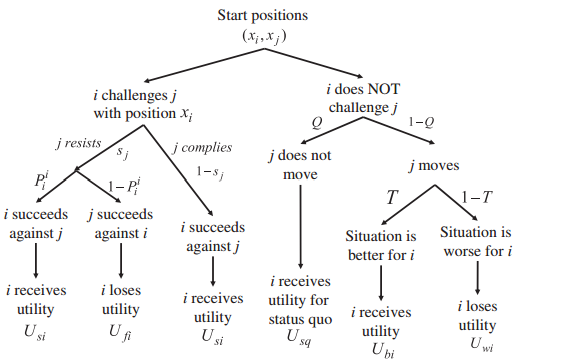
\includegraphics[height=9cm]{gametree.png}

\inputminted[fontsize=\footnotesize]{python}{bdm.py}

Bu yaklaşımı örnek olarak 1998'de Britanya'nın Avro para birliğine girip
girmeyeceği kararı üzerinde uygulayalım [6]. Alttaki değerler İşçi Partisinin
iktidarda olduğu senaryosuna göre seçilmiş, Muhafazakar iktidarı seçeneğinde
sadece aktörlerin gücü / etkileri değişiyor, pozisyonlar her iki durumda da
aynı. Skalada güç 0-1 arası, pozisyon 0-10.

\begin{minted}[fontsize=\footnotesize]{python}
import pandas as pd
dfuk = pd.read_csv('uk_emu_labor.csv'); print dfuk
\end{minted}

\begin{verbatim}
                       Actor  Capability  Position  Salience
0      Isci Partisi (Avrocu)         1.0         8        40
1  Isci Partisi (AB Karsiti)         0.5         4        40
2     Ingiliz Merkez Bankasi         0.1         5        60
3               Teknokratlar         0.1        10        40
4                Sanayiciler         0.1         5        40
5      Direktorler Enstitusu         0.1         4        40
6                Finanscilar         0.1         9        60
7     Muhafazakar AB Karsiti         0.3         1        95
8   Muhafazakar AB Taraftari         0.3         6        50
\end{verbatim}

Oyunu isletince sonuc,

\begin{minted}[fontsize=\footnotesize]{python}
import bdm
bdm.run("uk_emu_labor.csv",iter=5)
\end{minted}

\begin{verbatim}
Isci Partisi (Avrocu) tarafina geciyor Sanayiciler
Isci Partisi (AB Karsiti) tarafina geciyor Finanscilar
Teknokratlar tarafina geciyor Sanayiciler
Direktorler Enstitusu tarafina geciyor Finanscilar
Finanscilar kaybediyor Sanayiciler
Muhafazakar AB Karsiti tarafina geciyor Sanayiciler
5.0
Isci Partisi (AB Karsiti) tarafina geciyor Isci Partisi (Avrocu)
Direktorler Enstitusu tarafina geciyor Isci Partisi (Avrocu)
5.0
5.0
5.0
5.0
\end{verbatim}

5 değeri çıktı, ki bu [6]'daki sonuca yakın. Eğer Muhafazakar Parti iktidarına
göre işletirsek,

\begin{minted}[fontsize=\footnotesize]{python}
import bdm
bdm.run("uk_emu_cons.csv",iter=5)
\end{minted}

\begin{verbatim}
Isci Partisi (Avrocu) tarafina geciyor Ingiliz Merkez Bankasi
Isci Partisi (AB Karsiti) tarafina geciyor Ingiliz Merkez Bankasi
Teknokratlar tarafina geciyor Ingiliz Merkez Bankasi
Direktorler Enstitusu tarafina geciyor Ingiliz Merkez Bankasi
Finanscilar tarafina geciyor Ingiliz Merkez Bankasi
Muhafazakar AB Taraftari tarafina geciyor Ingiliz Merkez Bankasi
1.0
Isci Partisi (Avrocu) tarafina geciyor Muhafazakar AB Karsiti
Isci Partisi (AB Karsiti) tarafina geciyor Muhafazakar AB Karsiti
Teknokratlar tarafina geciyor Muhafazakar AB Karsiti
Sanayiciler tarafina geciyor Muhafazakar AB Karsiti
Direktorler Enstitusu tarafina geciyor Muhafazakar AB Karsiti
1.0
Ingiliz Merkez Bankasi tarafina geciyor Muhafazakar AB Karsiti
Finanscilar tarafina geciyor Muhafazakar AB Karsiti
Muhafazakar AB Taraftari tarafina geciyor Muhafazakar AB Karsiti
1.0
1.0
1.0
\end{verbatim}

Sonuç 1, yani Avro'ya hiç destek yok. Bu pek beklenmez bir durum değil, çünkü
İngiltere'de Muhafazakarlar AB'ye zaten soğuk dururlar. Tarihten biliyoruz ki
Britanya Avro'ya girmedi, hatta bilindiği gibi 2016'da referandumda AB'den çıkma
kararı aldı!

Ödev: Britanya'nın AB'den çıkışını (Brexit) tahmini.  Mesquita'ya göre metotu
için gereken ham veriyi yeterince haberleri izleyen herhangi biri
yaratabilir. Aktörler herhalde üstteki örneğe yakın olur, halkın seçiminin bu
aktörlerin seçimini yansıttığı varsayılabilir. Sonuç ne olur?

İlk baştaki emisyon örneği,

\begin{minted}[fontsize=\footnotesize]{python}
import bdm
bdm.run("emission.csv",iter=10,xmin=4)
\end{minted}

\begin{verbatim}
Belgium tarafina geciyor France
Luxembourg orta noktada anlasiyor France
Ireland tarafina geciyor France
10.0
Belgium tarafina geciyor Netherlands
Luxembourg tarafina geciyor Netherlands
Ireland orta noktada anlasiyor Netherlands
7.0
Belgium tarafina geciyor France
Luxembourg tarafina geciyor France
Ireland orta noktada anlasiyor France
10.0
Belgium tarafina geciyor Netherlands
Luxembourg tarafina geciyor Netherlands
Ireland tarafina geciyor Netherlands
7.0
Belgium tarafina geciyor France
Luxembourg tarafina geciyor France
Ireland orta noktada anlasiyor France
10.0
Belgium tarafina geciyor Netherlands
Luxembourg tarafina geciyor Netherlands
Ireland tarafina geciyor Netherlands
7.0
Belgium tarafina geciyor France
Luxembourg tarafina geciyor France
Ireland orta noktada anlasiyor France
10.0
Belgium tarafina geciyor Netherlands
Luxembourg tarafina geciyor Netherlands
Ireland tarafina geciyor Netherlands
7.0
Belgium tarafina geciyor France
Luxembourg tarafina geciyor France
Ireland orta noktada anlasiyor France
10.0
Belgium tarafina geciyor Netherlands
Luxembourg tarafina geciyor Netherlands
Ireland tarafina geciyor Netherlands
7.0
\end{verbatim}

Yeni Model

BDM'in yeni modeli yeni parametreler kullanıyor, örnek \verb!mugabe-full.csv!
içinde bulunabilir. Uzun yıllar başta kalan bir diktatör Mugabe'nin nasil o
noktada kalabildiğini destekcileri uzerinden görmek mümkün, bir türlü gitmek
bilmeyen liderlerin arkasındaki dinamikleri anlamak için bilgilendirici
herhalde!

Hocanın yeni modeli [4,9]'ta anlatılıyor fakat, kodlamak için hala yeterli bilgi
yok. Aslında eski kod için de yeterli bilgi yok, fakat [10]'daki araştırmacı
kolları siyayıp tüm makalelerde anlatılanları birleştirerek bir kod çıkartmaya
uğraşmış. Bir örneği \verb!masad/emissions.py!  içinde bulabiliriz.

Kaynaklar 

[1] Stack Exchange, {\em Expected Utility Method and a Repeated Game Solution}, \url{http://math.stackexchange.com/questions/1366279/expected-utility-method-and-a-repeated-game-solution}

[2] Bueno De Mesquita BB (1994) {\em Political forecasting: an expected utility
method}. In: Stockman F (ed.) {\em European Community Decision Making}. Yale, CT:
Yale University Press, Chapter 4, 71-104.

[3] Scholz, {\em Unravelling Bueno De Mesquita's group decision model},
\url{https://oficiodesociologo.files.wordpress.com/2012/03/scholz-et-all-unravelling-bueno-de-mesquita-s-group-decision-model.pdf}

[4] {\em A New Model for Predicting Policy Choices: Preliminary Tests}
\url{http://irworkshop.sites.yale.edu/sites/default/files/BdM_A%20New%20Model%20for%20Predicting%20Policy%20ChoicesREvised.pdf}

[5] Eftekhari, {\em Preana: Game Theory Based Prediction with Reinforcement Learning}, \url{http://www.scirp.org/journal/PaperDownload.aspx?paperID=49058}

[6] {\em The Predictability of Foreign Policies}, The British EMU Policy,
\url{https://www.rug.nl/research/portal/files/3198774/13854.pdf}

[7] J. Velev, Python Code, \url{https://github.com/jmckib/bdm-scholz-expected-utility-model.git}

[8] {\em The Visible Hand}, \url{http://s3.amazonaws.com/os_extranet_files_test/27236_59690_fa12visible.pdf}

[9] Mesquita, {\em The Predictioneer's Game}

[10] Masad, {\em Replicating the replication of BDM's Expected Utility Model}, \url{https://github.com/dmasad/BDM_DecisionModel_Replication}



\end{document}
